\documentclass[7pt,a4]{scrartcl}
\usepackage[landscape,margin=20pt]{geometry}

\usepackage{amsmath}
\usepackage{amssymb}
\usepackage{multicol}
\usepackage{graphicx}




%Commands to format and shorten
\setlength{\columnseprule}{0.2pt}
\setlength{\parindent}{0cm}
\setlength{\parskip}{-0.3em plus 0.2em}%plus 0.1ex minus 0.2ex}
\pagestyle{empty} 



\begin{document}
\begin{multicols}{4}
\section{Bianchi}

\subsection{probabilities}
$\pi$, probability of transmission, $p$, probability of collision,
$b_{i,k}$ stationary probability of state $i,k$:
\begin{align*}
p &= 1-(1-\pi)^{N-1} \\
\pi &= \frac{2}{ 1 + W_\textrm{min} + pW_\textrm{min}\sum^{m-1}_{k=0}(2p)^k}\\
	 &= \frac{2(1-p)}{(1-2p)(W_{min} + 1)+pW_{min}(1-(2p)^m)}\\
b_{i,k} &= \frac{CW_i - k}{CW_i} \cdot \left \{ \begin{array}{ll}
    (1-p) \sum_{j=0}^m b_{j,0} & i = 0\\
    p \cdot b_{i-1,0} & 0 < i < m\\
    p \cdot (b_{m-1,0} + b_{m,0}) & i = m
    \end{array} \right.
\end{align*}

\subsection{Saturation throughput}

\begin{align*}
 \tau &= \frac{E\lbrack\textrm{Payload Transmitted by user i in a slot time}\rbrack}{E[\textrm{Duration of slot time}]} \\ 
 &= \frac{P_\textrm{s}P_{\textrm{tr}}L}{P_\textrm{s}P_{\textrm{tr}}T_{\textrm{s}} + P_\textrm{tr}(1-P_\textrm{s})T_\textrm{c} + (1-P_\textrm{tr})T_\textrm{id}}, \\
 P_\textrm{s} &= \frac{N\pi (1-\pi)^{N-1}}{1-(1-\pi)^N}, \\
 P_\textrm{tr} &= 1-(1-\pi)^N, \\
 T_\textrm{s} &= t_\textrm{header} + t_\textrm{payload} + \textrm{SIFS} + t_\textrm{ACK} + \textrm{DIFS} + \sigma,\\
 T_\textrm{c} &= t_\textrm{header} + t_\textrm{payload} + \textrm{SIFS} + \sigma
\end{align*}

\section{Trunk dimensioning}
For a trunk of $N$ channels, an offered load $A=\lambda E[X]$, $X$ the call duration, $Y$ the call arrival per sec $\sim$ Poisson($\lambda$) 
\begin{align*}
	P_\textrm{Blocking} &= P(\textrm{Drop a call because busy line})  \\
	&= \frac{A^N}{N!\sum^N_{i=0}(\frac{A^i}{i!})}
\end{align*}

Each channel carries the traffic 

\begin{equation*}
	\rho = \frac{(1 - P_\textrm{blocking})A}{N}
\end{equation*}

\paragraph{Cellular efficiency} $E = \frac{Conversations}{cells\times MHz}$

\section{Cellular Geometry: Hexagons}

\textbf{Area}: $A=1.5R^2\sqrt{3}$\\
\textbf{Distance btw. adjacent cells}: $d=\sqrt{3}R$

\subsection{Co-channel interference}
\begin{description}
\item[Co-channel reuse ratio]: $Q = \frac{D}{R} = \sqrt{3N}$ with $D$ the \textbf{distance} to the nearest co-channel cell, $R$ the \textbf{radius} of a cell and $N$ the \textbf{cluster size}.

\item[Signal to Interference ratio (SIR)]: $\textrm{SIR} = \frac{S}{I} = \frac{S}{\sum^{i_0}_{i=1}I_i}$. With $S$ the desired signal \textbf{power}, $I_i$ the \textbf{interference power} from the $i$th interfering co-channel base-station, $i_0$ the \textbf{number of co-channel} interfering cells.

\item[Signal to Interference plus Noise ratio (SINR)] : SINR $= \frac{S}{I + N_0}$

\item[Average received power $P_r$]: $P_r = P_0(\frac{d}{d_0})^{-\alpha}$ or \\ 
$P_r(\textrm{dBm}) = P_0(\textrm{dBm})-10\alpha\log(\frac{d}{d_0})$ with $P_0$ the power received from a small distance $d_0$ from the transmitter and $\alpha$ the path loss exponent.
	
\item[SIR in the corner of a cell]: $\frac{S}{I} = \frac{R^{-\alpha}}{\sum^{i_0}_{i=1}D_i^{-\alpha}}$

\item[First interfering layer approximation]: $\frac{S}{I} = \frac{(\frac{D}{R})^\alpha}{i_0} = \frac{(\sqrt{3N})^\alpha}{i_0}$ eg. $=(\frac{D}{R})^2\frac{1}{2}$ for two first layer interferers (cell divided into 3 sectors with directional antennas.)

\end{description}

\subsection{Capacity of a cellular network}
For $B_\textrm{t}$ the total allocated spectrum and $B_\textrm{c}$ the channel bandwidth: 
\begin{align*}
m = \frac{B_t}{B_c \frac{Q^2}{3}} = \frac{B_t}{B_c\left(\frac{6}{3^{\frac{\alpha}{2}}}\left(\frac{S}{I}\right)_\textrm{min}\right)^{\frac{2}{\alpha}}}
\end{align*}
For a cluster size $N$, $N = (i + j)^2 - ij$ for $i,j=0,1,2,\ldots$ and number of channels $C$ we have $m=\lfloor\frac CN\rfloor$

\subsubsection{CDMA Capacity: single cell case}
For the bitrate $R$, available bandwidth $W$, noise spectral density $N_0$, thermal noise $\eta$, received user signal (at base station) $S$, we have a possible number $N$ of users:
\begin{align*}
	N = 1 + \frac{W/R}{E_b/N_0} - (\frac{\eta}{S})
\end{align*}
With a duty cycle $\delta$ (Discontinuous transmission mode: takes advantage of
intermittent nature of speech):
\begin{align*}
	N = 1 + \frac1\delta\frac{W/R}{E_b/N_0} - (\frac{\eta}{S})
\end{align*}
And if we have $m$ sectors, the effective capacity becomes $mN$
\subsubsection{CDMA multiple cells}
\paragraph{Frequency reuse factor on the uplink} 
$f = \frac{N_0}{N_0 + \sum_iU_iN_{ai}}$ where $N_0$ = total interference power received from $N-1$ in-cell users, $U_i$ = number of users in the$i^\text{th}$ adjacent cell and $N_{ai}$ = average interference power from a user located in the $i^\text{th}$ adjacent cell

\paragraph{Average received power from users in adjacent cell}
$N_{ai} = \sum_j N_{ij}/U_i$ where $N_{ij}$ = power received at the base station of interest from the $j^\text{th}$ user in the $i^\text{th}$ cell

\subsection{Propagation modes}
\begin{multicols}{2}
	\begin{description}
		\item[Ground Wave] : $f \le 2$ Mhz
		\item[Sky Wave]
		\item[Line of Sight] : $f \ge 30$ Mhz
	\end{description}
\end{multicols}

\subsection{Line of sight equations}
Horizon distance $d[\textrm{km}]$ in \textbf{kilometers}, antenna height $h[\textrm{m}]$ and refraction adjustment factor $K = 4/3$:
\begin{description}
\item[Optical LOS]: $d = 3.57\sqrt{h}$
\item[Effective LOS]: $d = 3.57\sqrt{Kh}$
\item[Max LOS distance for two antennas :] $$3.57(\sqrt{Kh_1}+ \sqrt{Kh_2})$$
\end{description}

\section{Noise}
\paragraph{Thermal Noise}$N_0 = kT\quad(W/Hz)$

For signal power $S$, bitrate $R$, $k = 1.3806\cdot10^{-23} JK^{-1}$ the Boltzmann constant and $T$ the temperature: $\frac{E_b}{N_0} = \frac{S/R}{N_0} = \frac{S}{kTR}$

%Include slide 26 of A2 (throughput expressions)? 
\section{Wireless Misc Stuff}

\paragraph{Network Layers} Top-down: Application, Transport, Network, Data-link, Physical.


\underline{Security Requirements}:
\textbf{Confidentiality, Authenticity, Replay Detection, Integrity, Access Control,Jamming Protection}

\subsection{Ad-hoc Netowrks} %D3 - slide 48
\paragraph{Upper Bound for the Throughput} 
If we have $n$ identical randomly located nodes each capable of transmitting $W$ bits/s. 
Then the throughput $\lambda(n)$ obtainable by each node for a randomly chosen destination is $\lambda(n) = \Theta\left(\frac W{\sqrt{n\log n}}\right)$

\subsection{Antennas \& Propagation}
Free space propagation, received power: $P_\textrm{R} = P_\textrm{T}\frac{A_\textrm{R}}{4\pi d^2}\eta_\textrm{R}$ with $\eta_\textrm{R}$ an efficiency parameter, $A_\textrm{R}$ the receiving antenna area.
\\
Focusing capability, depends on size in wavelength $\lambda$:  
\\$G_\textrm{T} = 4\pi\eta_\textrm{T}A_\textrm{T}/\lambda^2$ \\
Directional emitter, received power: $P_\textrm{R} = P_\textrm{T}G_\textrm{T}\frac{A_\textrm{R}}{4\pi d^2}\eta_\textrm{R}$

Free space received power: $P_\textrm{R} =  P_\textrm{T}G_\textrm{T}G_\textrm{R}(\frac{\lambda}{4\pi d})^2$

Loss: $L = \frac{P_T}{P_R} = \frac{(4\pi d)^2}{G_RG_T\lambda^2} $

$ c = 3 \cdot 10^8 $

Parabola: $G = \frac{7A}{\lambda^2}$

\underline{\textbf{Mobnet Decibels}}:
$B = 10\log(\frac{P}{P_0})$
\subsection{Free Space Loss}
%TODO PICKUP HERE
Free space loss, ideal isotropic antenna:
$$ \frac{P_t}{P_r} = \frac{(4\pi d)^2}{\lambda^2} = \frac{(4\pi fd)^2}{c^2} $$
Free space loss equation can be recast:
$$L_{DB} = 10\log \frac{P_t}{P_r} = 20 \log(f) +20\log(d) - 147.56 dB$$
Free space loss accounting for gain of other antennas: 
$$\frac{P_t}{P_r} = \frac{(4\pi d)^2}{G_rG_t\lambda^2} = \frac{(cd)^2}{f^2A_rA_t}$$
$G_t$ = gain of transmitting antenna\\
$A_r$ = effective area of receiving antenna

\subsection{Protocol performances}
$G$: Total load, $S$ arrival rate of new packets. 
\subsubsection{Pure ALOHA}
\begin{align*}
P(k \text{ transm. in } 2X\text s) &= \frac{(2G)^k}{k!} e^{-2G}\\
S = G \cdot P(0) &= Ge^{-2G}
\end{align*}

\subsubsection{Slotted ALOHA} 
%C'est pas slotted alpha ça? 
Probability of $k$ packets generated during a slot:

\begin{equation*}
P(k) = \frac{G^ke^{-G}}{k!}
\end{equation*}

Throughput:

\begin{equation*}
P(1) = Ge^{-G}
\end{equation*}

\subsubsection{CSMA}
\paragraph{Non-persistent} If channel is busy, directly run back off algorithm.
\paragraph{p-persistent} If it is busy, they persist with sensing until the channel becomes idle. If it is idle:\\
- With probability $p$, the station transmits its packet\\
- With probability $1-p$, the station waits for a random time and senses again

\paragraph{Performance of Unslotted nonpersistent CSMA}:
For $a=t_\textrm{prop}/X$, the normalized one-way propagation delay.

\begin{equation*}
S = \frac{G^{-aG}}{G(1+2a)+e^{-aG}}
\end{equation*}

\paragraph{Performance of Slotted nonpersistent CSMA}:

\begin{equation*}
S = \frac{aG^{-aG}}{1-e^{-aG} + a}
\end{equation*}

\subsection{DOMINO Cheating detection}
\begin{tabular}{|p{0.35\columnwidth}|p{0.55\columnwidth}|}
  \hline
  Cheating Method & Detection Test \\\hline
  Frame scrambling & Number of retransmissions \\
  Oversized NAV1 & Comparison of the declared and actual NAV values\\
  Transmission before DIFS & Comparison of the idle time after the last ACK with DIFS \\
  Backoff manipulation & Actual Backoff/ Consecutive Backoff \\
  Frame scrambling with MAC forging & Periodic dummy frame injection\\
   \hline
\end{tabular}

\subsection{Forward Error Correction (FEC)}
Redundancy in packets to allow limited error correction at the receiver: used in 802.11a (Convolutional), HSDPA (Turbo Codes) and 802.11n (LDPC).

\section{TCP}

\subsection{Standard}

\paragraph{Tahoe} Basic TCP. Three duplicate ACK's provoke fast retransmit (resend 1\textsuperscript{st} missing packet), set \texttt{ssthresh} to \texttt{cwnd/2}, \texttt{cwnd} to 1 and provoke slow start.

\paragraph{Reno} Three duplicate ACK's provoke fast retransmit, \texttt{ssthresh} to \texttt{cwnd/2}, \texttt{cwnd} to \texttt{ssthresh + 3} and enter fast recovery.

\subparagraph{Fast Recovery} Increase \texttt{cwnd} by 1 segment for every received duplicate ACK. (\underline{Warning, unlogical}: When new ACK is received, \texttt{cwnd = ssthresh} and enter congestion avoidance). If a timeout occurs, set \texttt{cwnd} to 1 and enter slow start.
\paragraph{New Reno Fast Recovery} More intelligent fast recovery where you remember the last received ACK.

\subsection{Mobile}
\paragraph{Indirect TCP (I-TCP)} Connection split at FA. Standard TCP on the wire line, wireless optimized TCP on the wifi side: shorter timeout, faster retransmission. Loss of end-to-end semantics, security issues.
\paragraph{Mobile TCP (M-TCP)} Split connection at FA. Monitor packets, if a disconnect is detected, report receiver window $= 0$: sender will go into persist mode and doesn't timeout or modify his congestion window. Preserves end-to-end semantics. Disadv.: wifi losses propagate to the wire network, link-errors pkt loss must be resent by sender, security issues. \underline{Summary}: only handles mobility errors, no transmission errors.

\paragraph{Snooping-TCP} TCP-aware link layer: Split connections, FA buffers and retransmits segments, does not ACK buffered packets (preserves end-to-end semantics).

\paragraph{Transaction oriented TCP (T-TCP)} TCP phases: connection setup, data transmission, connection release. T-TCP combines does steps and only 2-3 packets are needed for short messages. Efficient for single packet transactions, but requires TCP modifications on all hosts.

\section{Security}
\paragraph{GSM} Shared secret and challenge responses, one-way authentication.
\paragraph{3GPP} Two-way authentication.

\section{Privacy}
\paragraph{Privacy Related Notions}Anonymity, untraceability, unlinkeability, unobservability, pseudonymity
\paragraph{Best to worst against information leakage:}
GPS: no third-party, determined 'alone'.
Cell-ID: requires the operator database that is relatively protected (they won't easily mine you).
Wireless: requires one or several third-party owned databases that can track you, and it is relatively precise due to short radio range.

\subsection{Privacy Metrics}

\paragraph{Entropy-Based Anonymity}
$A$ the anonymity set, $p_x$ the probability for an external observer that the action was performed by $x$:
\begin{equation*}
	\sum_{\forall x \in A} p_x \log(p_x)
\end{equation*}

\paragraph{Entropy-Based Unlinkability}
$I_1,I_2$, sets of elements to be related, $p_r$, the probability two elements are related for an external observator:
\begin{equation*}
	\sum_{\forall R \subseteq I_1 \times I_2}p_r \log(p_r)
\end{equation*}

\subsection{RFID}
\paragraph{Singulation} (determining which tags are present around the reader) Binary tree walking: reader first asks the tags to emit the first bit of their ID. If every answer is 0 (or 1) the reader knows on which side the ID's are. This is done recursively until all ID's are determined.

\paragraph{Privacy zone} A tag ID can be changed so that it lies in the \emph{private} zone of the tree. A special device simulates collisions for every query in this area, so an exhaustive search would be required to find a tag. 

\paragraph{Pseudonyms} Tags can be set to use different ID's that an authorized reader would know how to correlate. To avoid having too complex tags, the reader will generally be responsible for \emph{refilling} the pseudonyms. This will be done in cleartext and assumes an attacker does not always listen.

\subsubsection{Key Tree}
Tags are the leaves of a tree with branching factor $b$ and depth $d$, and each edge to arrive to a tag has an associated key: hence, a tag has $d$ associated keys.
\begin{center}
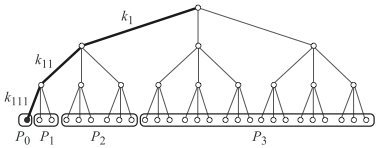
\includegraphics[width=0.7\columnwidth]{img/anon_set}
\end{center}

\paragraph{Anonymity set} has minimum size of 1, maximum size of all the tags. Compromising a tag yields all the keys leading to it and permit to partition the other tags (neighbors in the tree share common keys) : $P_0$ contains the compromised tag, $P_1$ contains the compromised tag's \emph{brothers} not being in $P_0$, etc. Tags that belong to larger partitions have better privacy (e.g: tags in $P_3$ are not distinguishable, attacker only knows they don't use $k_1$.)

\paragraph{Expected size of the anonymity set for a random tag}: for $n$ the total number of tags and $|P_i|/n$ the probability of selecting a tag from partition $P_i$

\begin{equation*}
\bar S = \sum_{i=0}^d \frac {|P_i|}n|P_i| =  \sum_{i=0}^d \frac {|P_i|^2}n
\end{equation*}

\paragraph{Normalized expected anonymity} : 
Using $n = b^d$ and $|P_0| = 1, |P_1| = b-1, |P_2| = (b-1)b, \ldots, |P_l| = (b-1)b^{l-1}$.
\begin{equation*}
	\frac{\bar{S}}n = \sum_{i=0}^d \frac {|P_i|^2}{n^2} = \frac{b-1}{b+1} + \frac2{(b+1)n^2}
\end{equation*}

For \textbf{one} tag in $P_i$, the linkability probability is  $1/|P_i| \rightarrow$ global linkability in $P_i$ is $|P_i|\frac1{|P_i|} = 1$. For $l$ partitions, the probability that two transactions from a randomly chosen tag are linkable is:

\begin{equation*}
\frac1n\sum_{i=1}^l(|P_i|\frac1{|P_i|}) = \frac ln
\end{equation*}
With $n = b^d$

\end{multicols}
\end{document}



